% !TEX root = ../thesis-example.tex
%
\chapter{Implementation}
\label{sec:concepts}

\section{Log In and Registration}
Log in and registration GUI are shown in the following. When registering user needs to specify their role. After registering user can log into the system using the email and password.

\begin{figure}[h]
\centering
\begin{subfigure}{.5\textwidth}
  \centering
  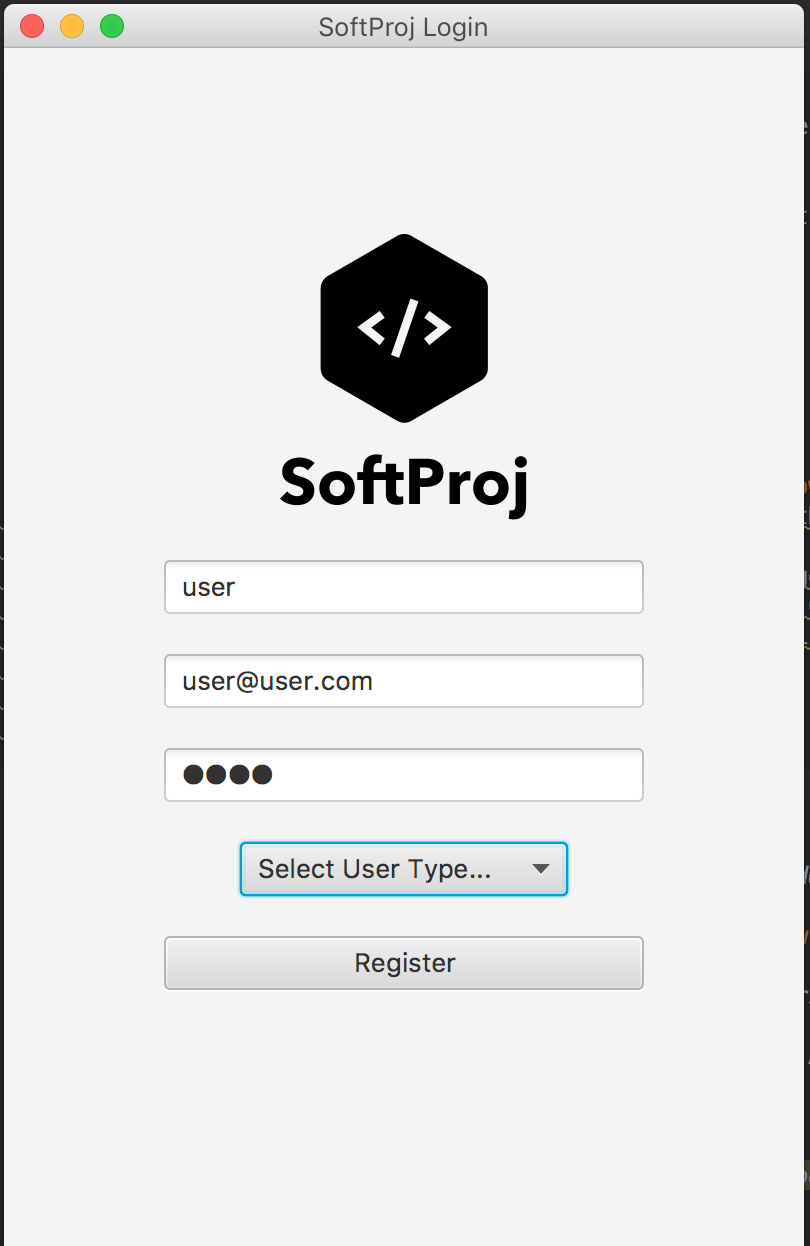
\includegraphics[width=.6\linewidth]{content/1.png}
  \caption{}
  \label{fig:sub1}
\end{subfigure}%
\begin{subfigure}{.5\textwidth}
  \centering
  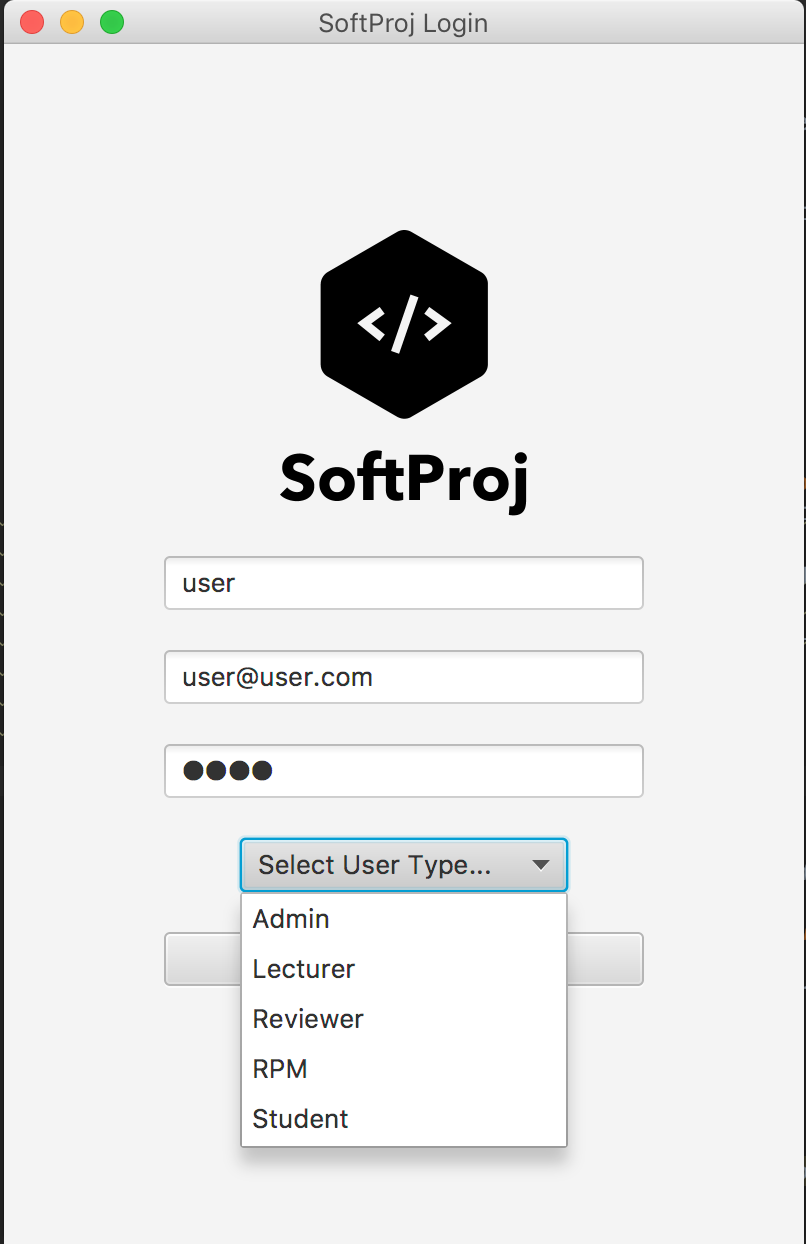
\includegraphics[width=.6\linewidth]{content/2.png}
  \caption{}
  \label{fig:sub2}
\end{subfigure}
\caption{Creating account in the system}
\label{fig:test}
\end{figure}


\begin{figure}[h]
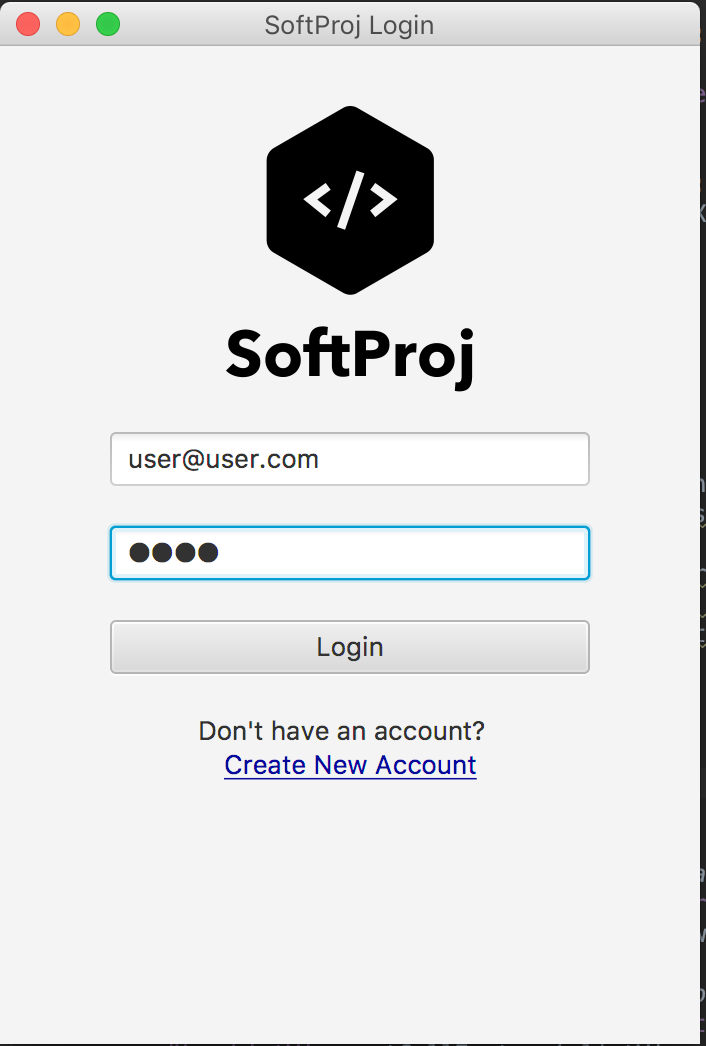
\includegraphics[width=4cm]{content/3.png}
\centering
\caption{Logging into the system}
\end{figure}


\section{Graphical User Interface(GUI) for Student}

\begin{figure}[h]
\centering
\begin{subfigure}{.5\textwidth}
  \centering
  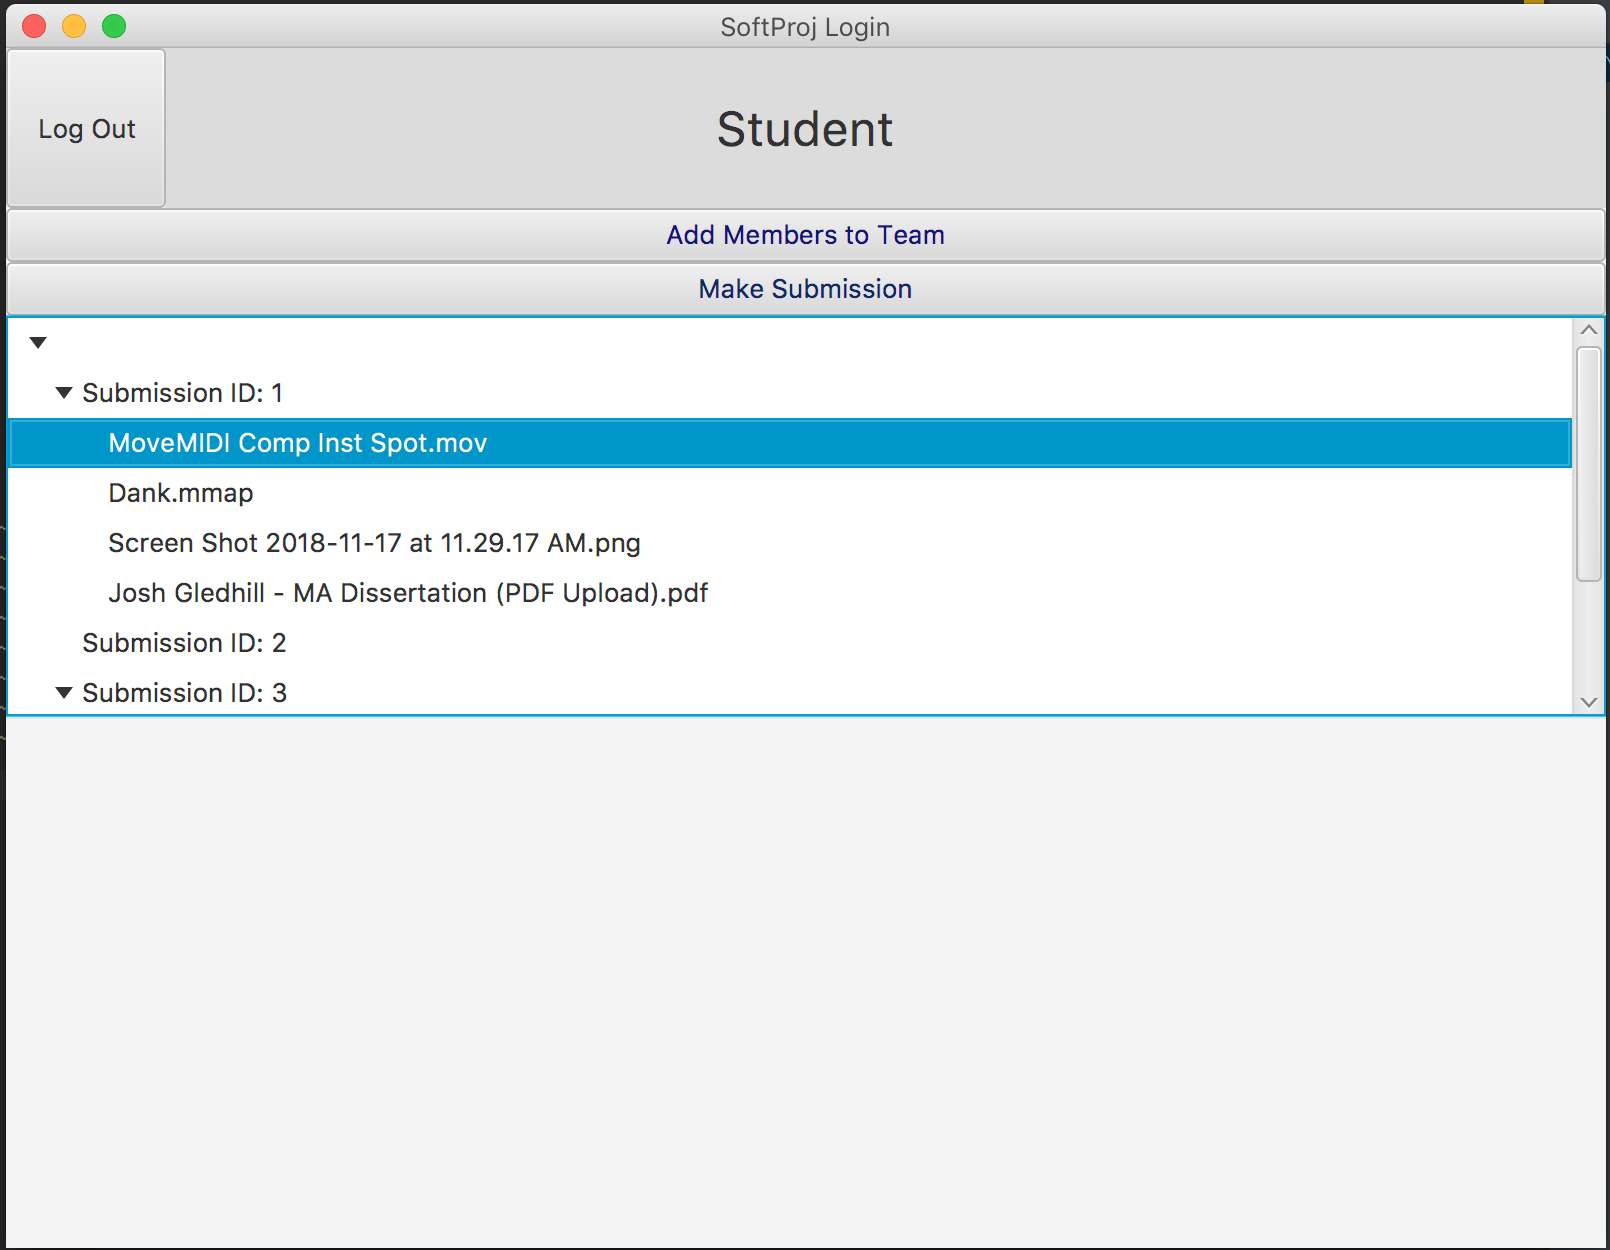
\includegraphics[width=.8\linewidth]{content/5.png}
  \caption{}
  \label{fig:sub1}
\end{subfigure}%
\begin{subfigure}{.5\textwidth}
  \centering
  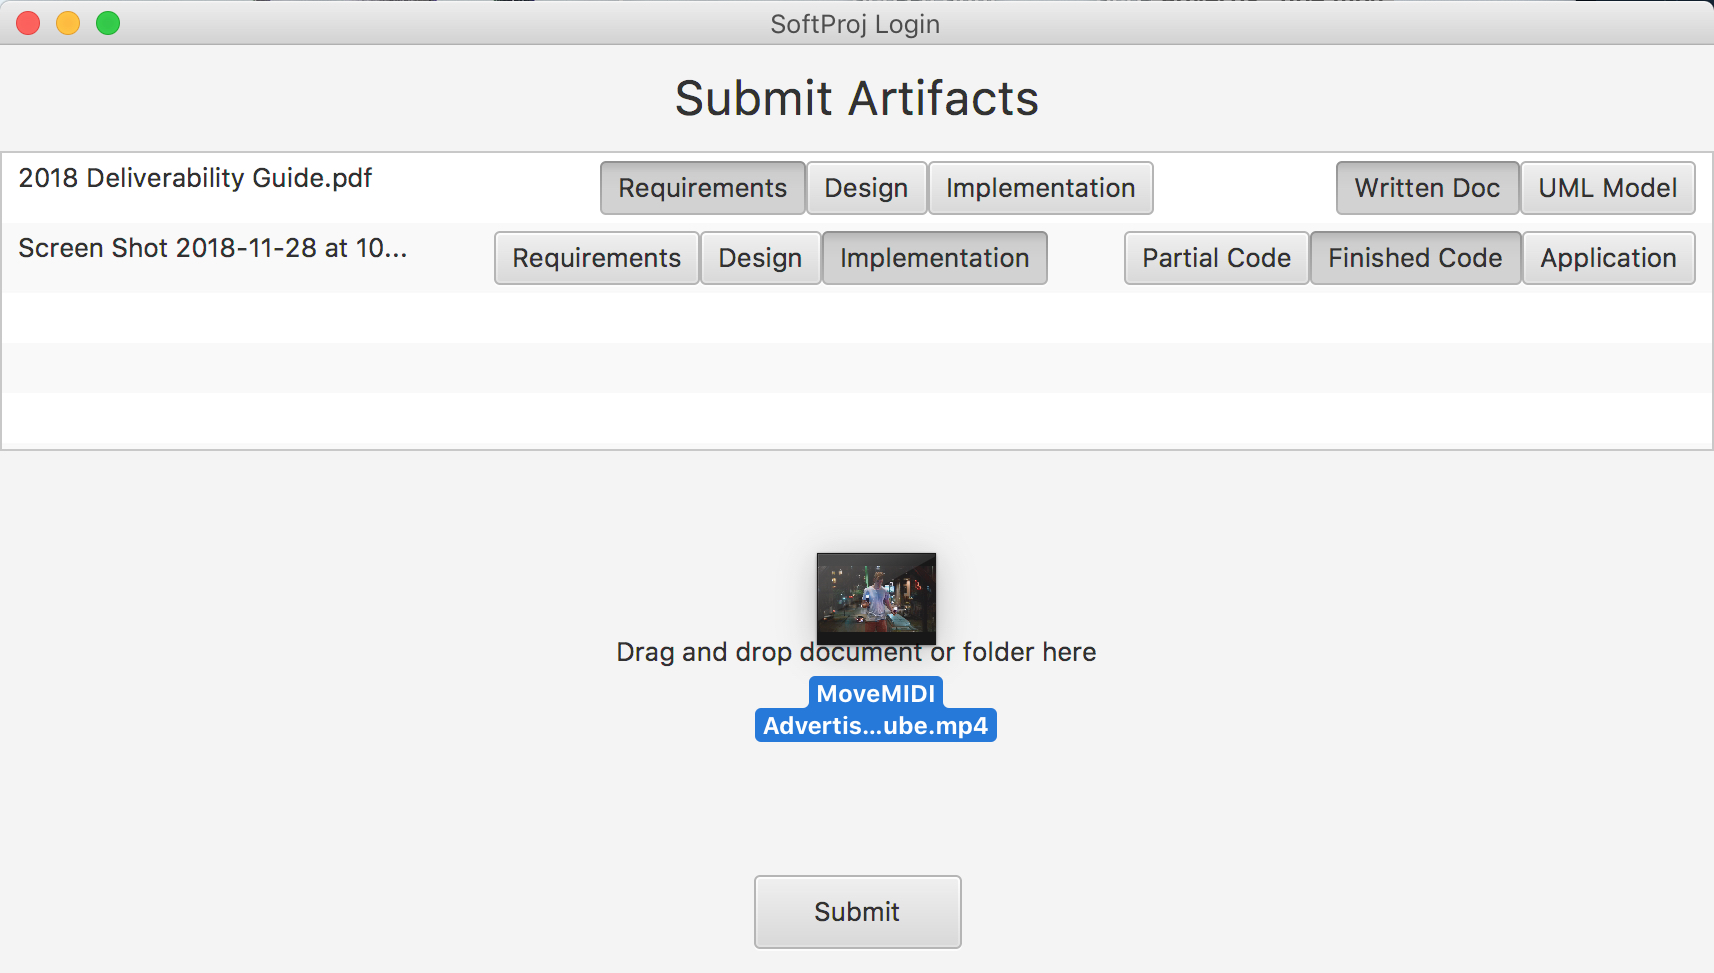
\includegraphics[width=1\linewidth]{content/10.jpg}
  \caption{}
  \label{fig:sub2}
\end{subfigure}

\begin{subfigure}{.5\textwidth}
  \centering
  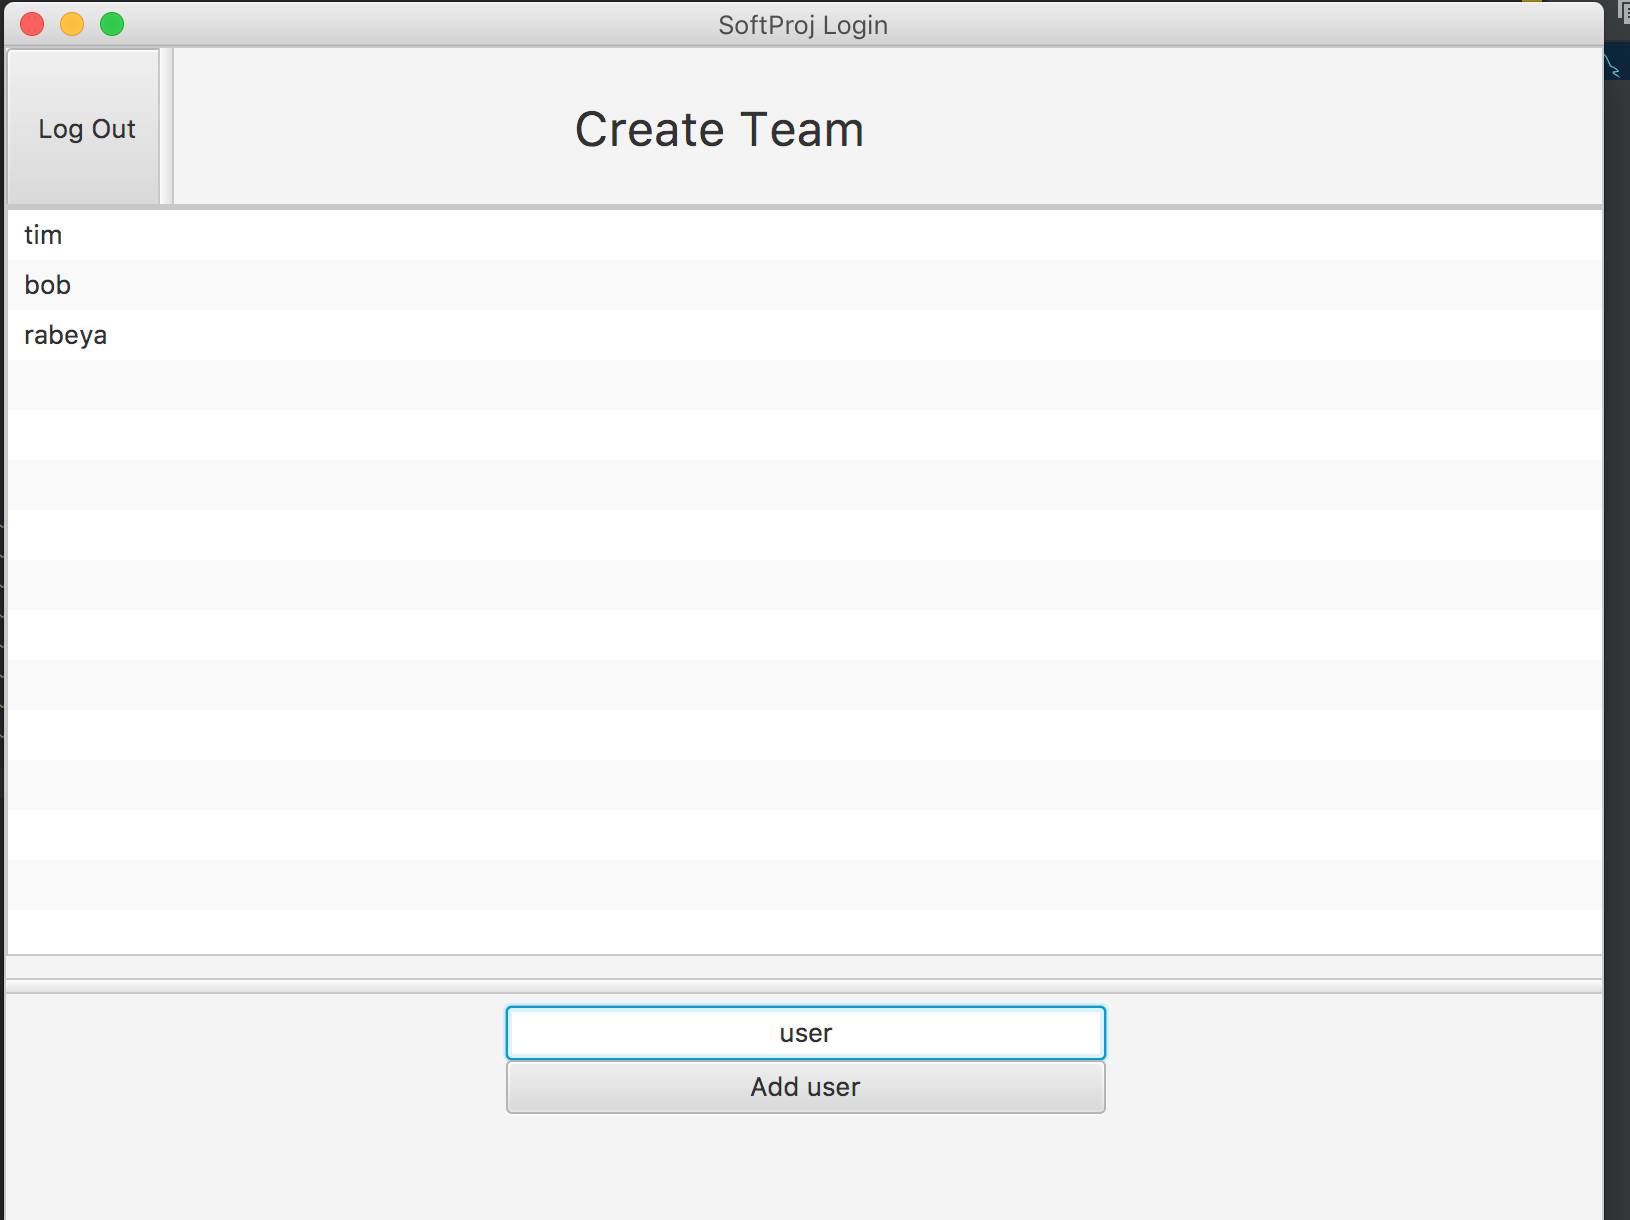
\includegraphics[width=1\linewidth]{content/6.png}
  \caption{}
  \label{fig:sub2}
\end{subfigure}
\caption{Logging into the system as Student}
\label{fig:test}
\end{figure}

Figure 4.3(a) shows the GUI when a student logs into the system. He/She can see the previous submitted artifacts and their status. Figure 4.3(b) shows how to submit artifacts.Figure 4.3(c) shows the GUI if a student wants to create team.
\newpage

\section{Graphical User Interface(GUI) for Lecturer}
 Following is the GUI for Lecturer. As shown in the figure, Lecturer can see the both the artifacts that are reviewed and that need to be reviewed.He/She can also see the list of the teams and reviewers.


\begin{figure}[h]
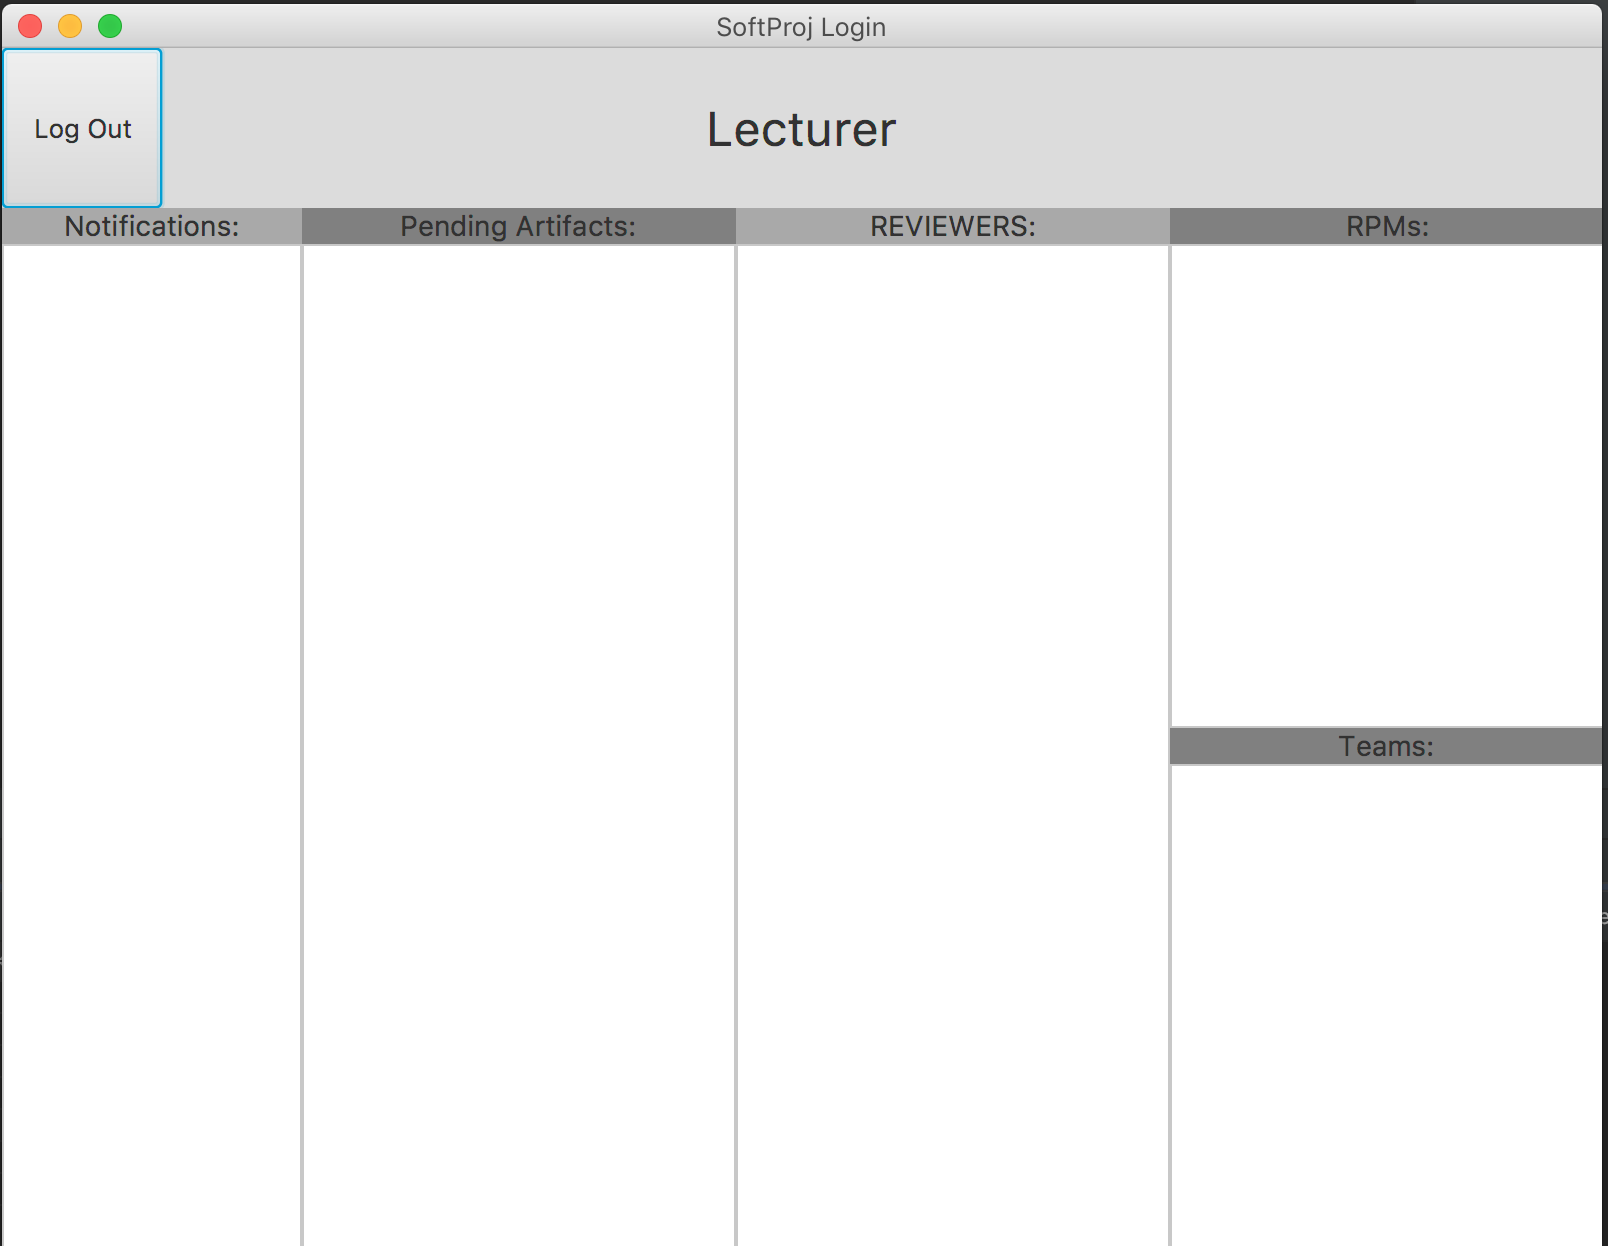
\includegraphics[width=7cm]{content/8.png}
\centering
\caption{Logging into the system as Lecturer}
\end{figure}



\section{Graphical User Interface(GUI) for RPM}
 Following is the GUI for RPM. As shown in the figure, RPM can see the progress of his/her works and the new artifacts that need to be assigned to Reviewer.


\begin{figure}[h]
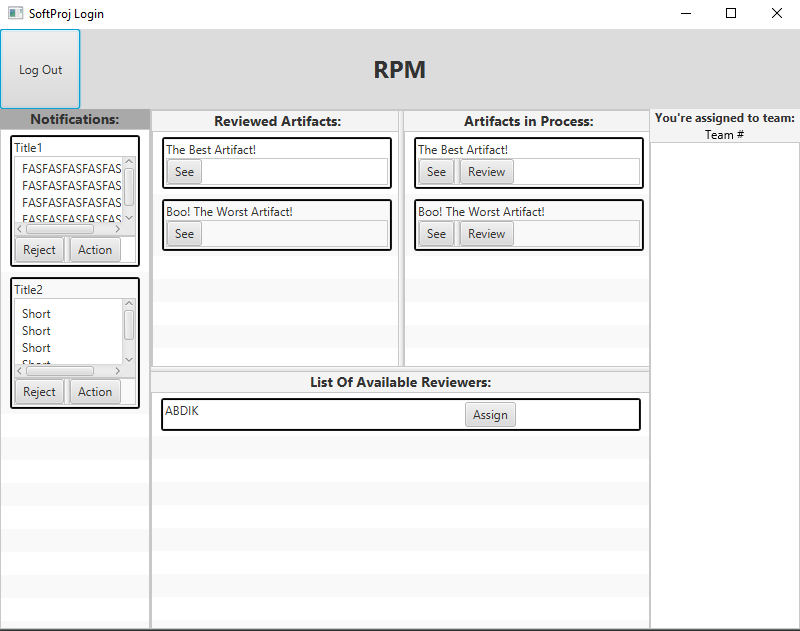
\includegraphics[width=9cm]{gfx/RPM.png}
\centering
\caption{Logging into the system as RPM}
\end{figure}




\section{Graphical User Interface(GUI) for Reviewer}
 Following is the GUI for Reviewer. As shown in the figure, Reviewer can see the progress of his/her works and the new artifacts that need to be reviewed.


\begin{figure}[h]
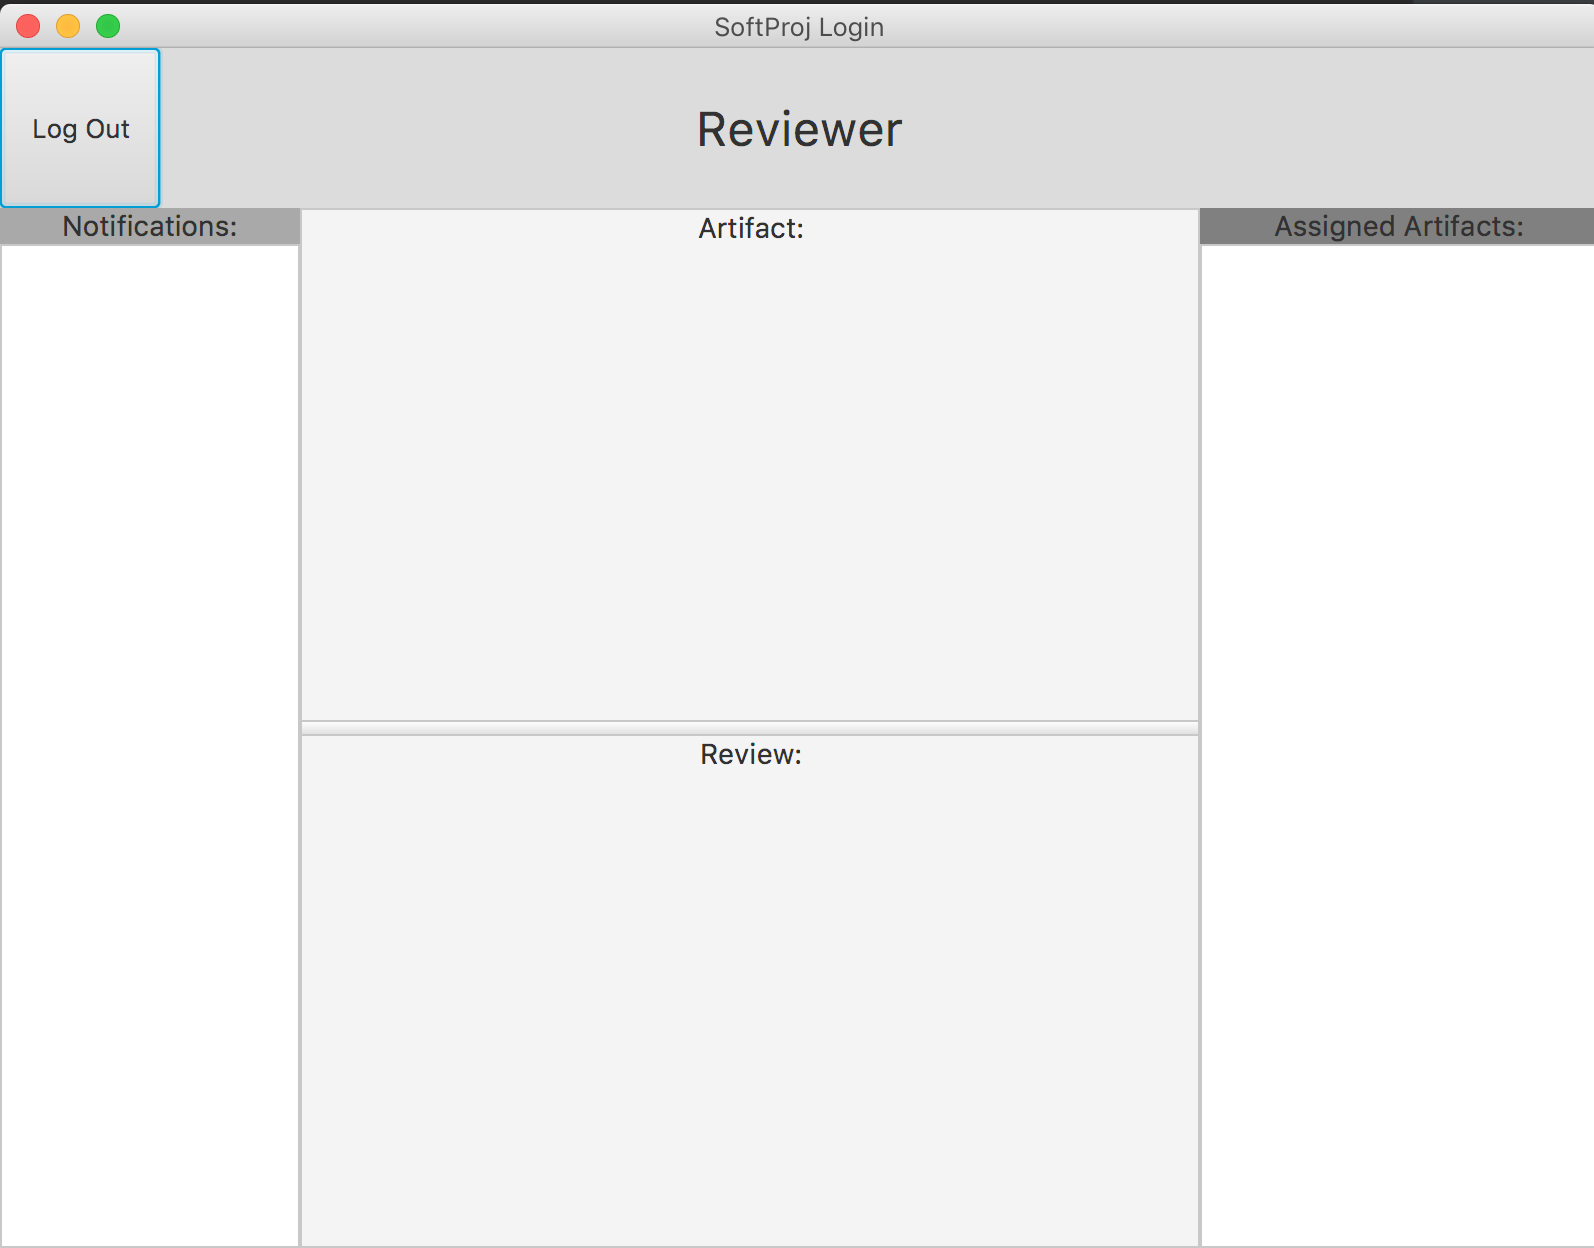
\includegraphics[width=9cm]{content/9.png}
\centering
\caption{Logging into the system as Reviewer}
\end{figure}





\section{Graphical User Interface(GUI) for Admin}
 Following is the GUI for Admin. As shown in the figure, Admin can approve, modify and delete the accounts.Admin can also see all the artifacts.


\begin{figure}[h]
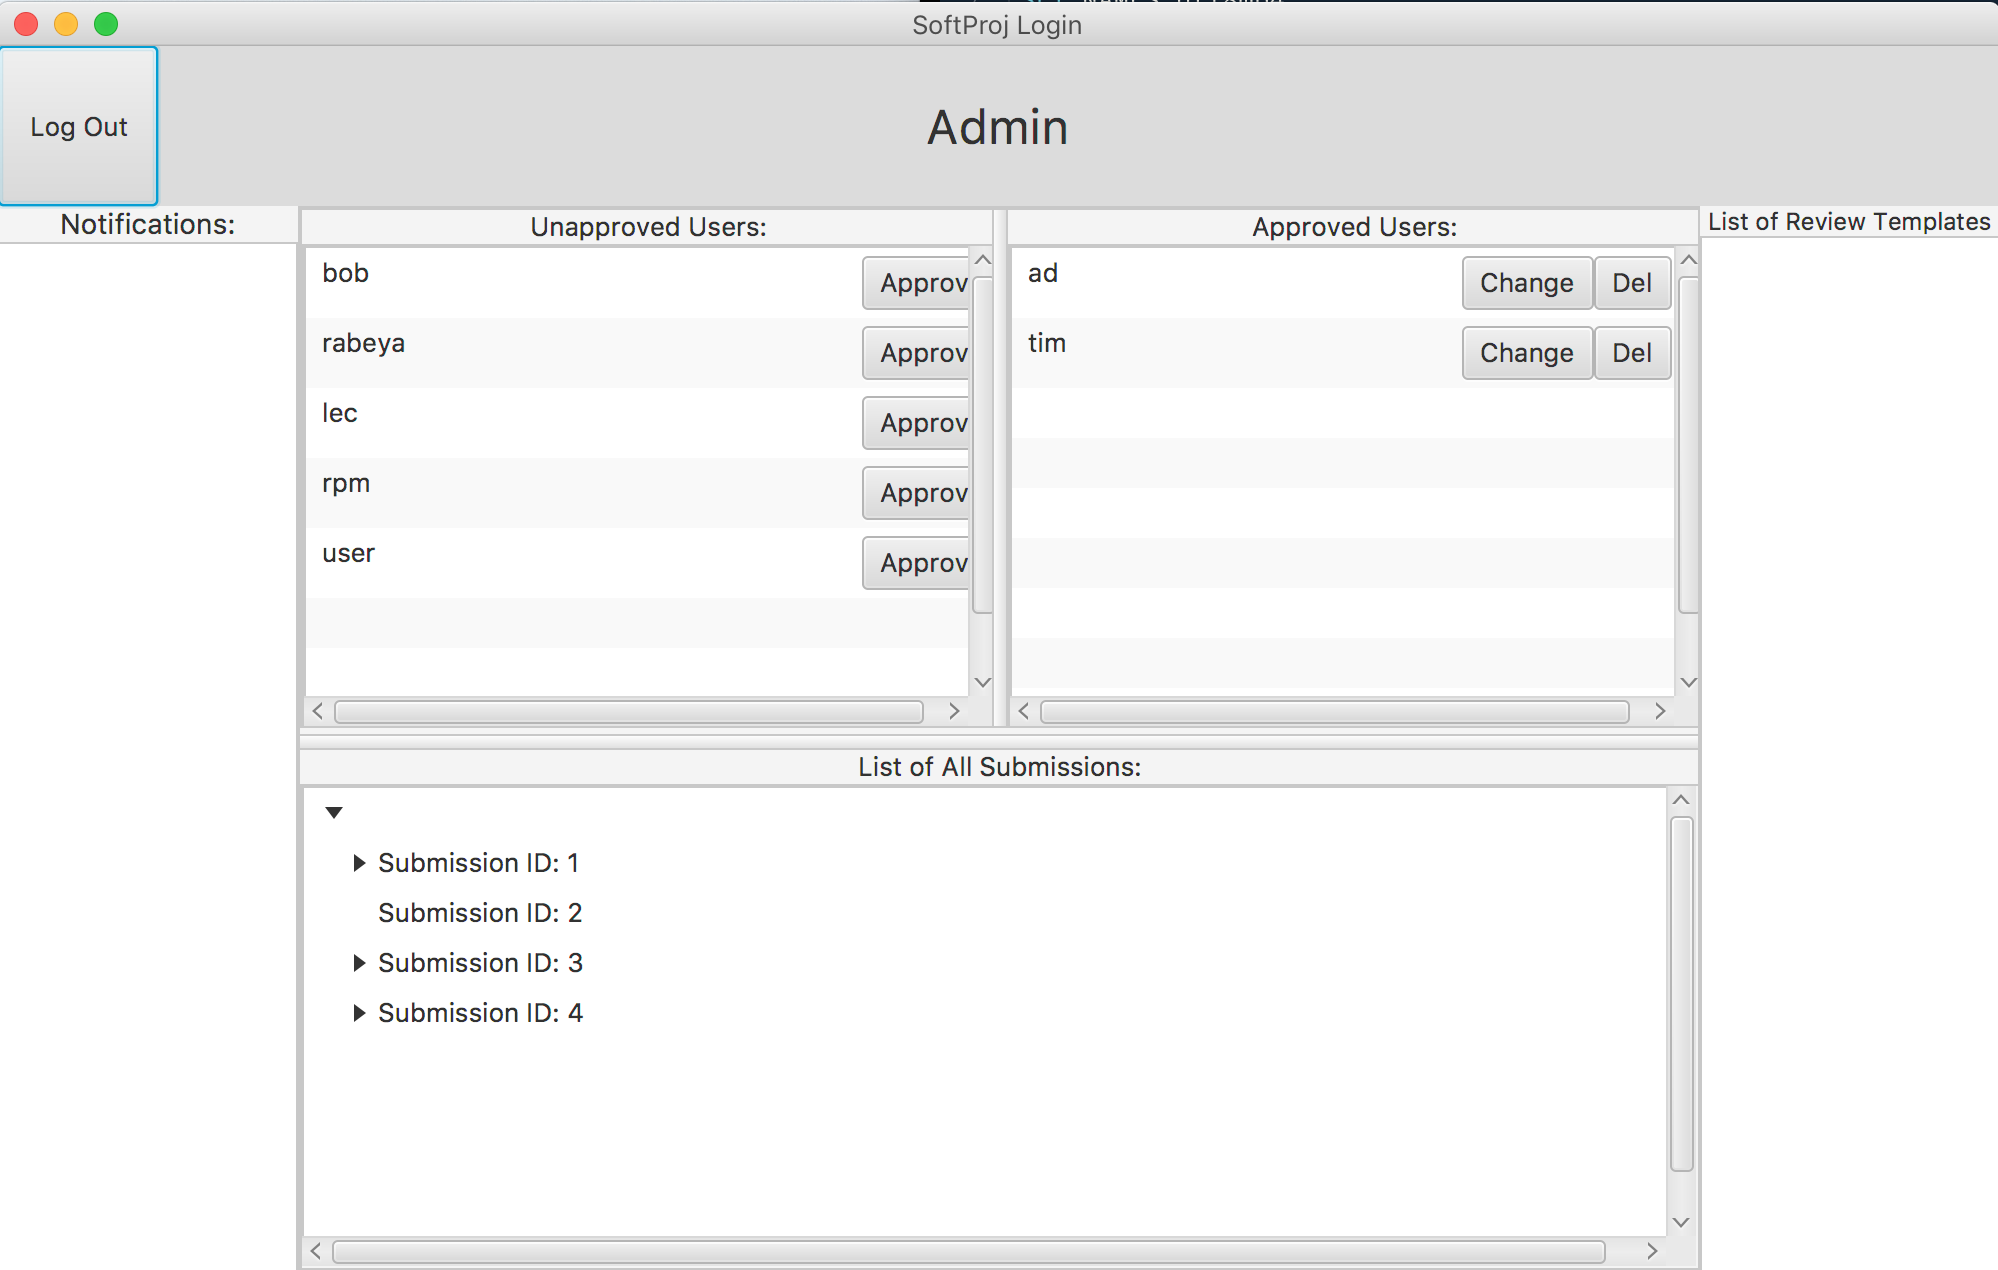
\includegraphics[width=9cm]{content/7.png}
\centering
\caption{Logging into the system as Admin}
\end{figure}









